\section{2016-01-08 Interaction Designer Interview}

\begin{figure}[h]
\centering
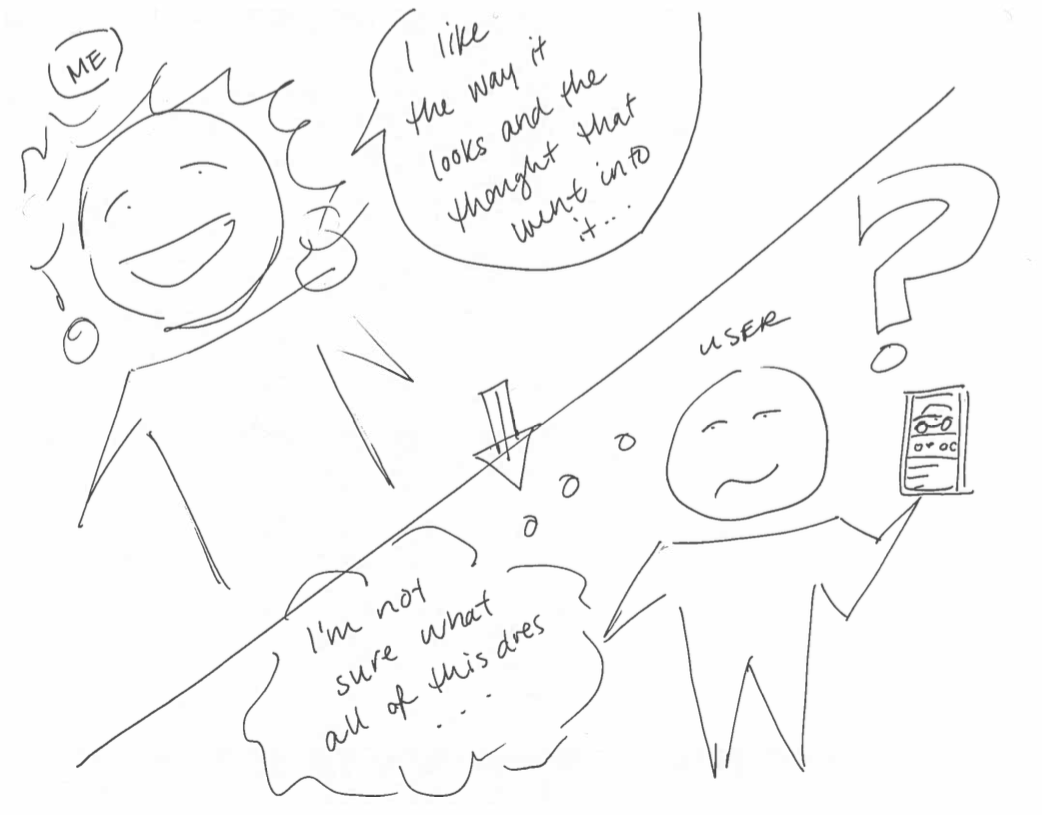
\includegraphics[width=6.5in]{interviews/drawings/2016_01_08.png}
\caption{\quotes{2016-01-08 Interaction Designer's drawing of software development process}}
\label{2016_01_08}
\end{figure}

\textbf{Todd:} My first question for you is very open ended.  00:02

\textbf{Interviewee:} Okay.  00:03

\textbf{Todd:} There is no wrong answer.  I was hoping if you could draw how you feel about the product.  00:09

\textbf{Interviewee:} Okay.  This may get elaborate.  00:27

\textbf{Todd:} Fantastic.  00:29

\textbf{Interviewee:} This is my new pen so.  [Pause] Here we are.  I did sort of a story board-ish type of thing.  02:54

\textbf{Todd:} I love it.  02:55

\textbf{Interviewee:} So, do you want me to explain it?  02:58

\textbf{Todd:} Please.  02:58

\textbf{Interviewee:} Okay.  On one hand superficially, I'm happy because aesthetically, I think it's nice.  I think it's, when you compare it to some of the projects we do, it's been going on for so long and there's such a huge team of smart people.  I feel like we got so much done and it's complex and interesting and there's lot of thought that went into it and it's a really robust app but I'm worried that even though it's pretty and we built a lot of features and the technology is cool, not all of it is necessarily useful for end users and I didn't even give the user name anything because I don't even know that we're designing for the right person all the time with some of our features .  I don't know.  So, I'm worried there were will be more confusion in the marketplace than I would like there to be in a product that I've worked on.  03:57

\textbf{Todd:} Anything else?  04:01

\textbf{Interviewee:} In the drawing or in general?  04:05

\textbf{Todd:} Both.  04:06

\textbf{Interviewee:} Not so much in the drawing.  I guess the big question mark is just that I don't know, I think it's pretty usable but I'm worried there's going to be features like predictive for the users or going to be like what is this or why do I care or they'll have question marks around there's something really obvious to me like \ldots I would like you heard a lot of feedback, I want a light telling me if my oil is low and that's just not something we could do because of constraints on the technology I think.  So, I'm worried if people will look at it and say why is there all this stuff that I don't want and there's some stuff that maybe feels really obvious to some users that we haven't provided for one reason or another but overall, I still feel happy.  I think we created a solid product.  04:59

\textbf{Todd:} Good.  When you were describing your \quotes{you} picture, you used the word superficially.  I don't remember the exact word but something like given this superficially I feel happy about it and I was curious if there was like an under feeling of the product.  05:17

\textbf{Interviewee:} Yeah, currently to some degree, this is the under feeling.  The superficial part is a little bit as a designer is a normal person walking around, you feel like people look at it and like it's so beautiful and that might be the beginning and the end of what they think of the app.  They might not use it.  Maybe, it's not for them.  I feel like I could put it in a portfolio or take some of those App Store screens and show it to people and maybe like oh my God, this is the nicest product, you must have done a great job or your team must have worked really hard but if we built something that's really beautiful but doesn't meet the needs of our users, it's kind of I'm still superficial.  I guess part of me is still happy it's beautiful at least or that there's parts of it that are really pretty but at the end of the day as a designer, it's kind of a big fail to build something that's pretty but not the right thing.  It should be a big fail for everybody but especially as the designer, that's what you want to avoid.  06:21

\textbf{Todd:} Yeah.  So, what do you do with that tension?  06:25

\textbf{Interviewee:} During the life cycle of a product, one of the things we enable people on or if you work some more even not as a consultant, I feel like a part of your job as a designer is to constantly be educating everyone else that things that look pretty but don't work are bad designs.  I think design isn't about just making it pretty.  It's really more about making it useful.  And so, that's something that I think is a big part of our design enablement here that we work on consistently now that I'm rolling off the project.  It kind of is what it is.  I guess if I was staying on the project longer, I would keep pushing and I think the design team as a whole would keep pushing back on features that we don't think meet our user's needs and keep pushing for features that we think might not be as popular from a business perspective but would be popular with Hannah and Michael.  07:35

\textbf{Todd:} How does this affect \ldots well this is your last day.  How has this affected your motivation for the product or for the project?  07:44

\textbf{Interviewee:} Not negatively.  This is \ldots I guess I'm happy face because even though I have some question marks about some of the features, we had to prioritize and how you solve that.  There's still things we fought for that weren't on our original feature list and actually got to put in.  We did research and we know these features are going to be popular with our users and that's a huge win and also happy because I'd rather make something that looks polished or looks good even if it's not perfect functionality than something that doesn't have all perfect functionality and looks bad.  So at least if it's beautiful or elegant or it feels sexy to some users that's still your part way there.  It's just not the whole picture.  08:39

\textbf{Todd:} Cool.  So, it sounds like your motivation is either intrinsic or extrinsic.  It's outside of like I don't know is it the product set or the features or the \ldots I'm trying to ask.  Yeah, I guess what motivates you when you think about you as a designer.  08:59

\textbf{Interviewee:} I think it's more intrinsic which is why I'm happier being a designer than some of my past jobs and I think part of it is the process of building something or making something.  I really enjoy that starting with nothing and you know at the end, there's something out there that wasn't there before.  I find that kind of creative, creating and build process really satisfying.  I like the problem solving.  I think I'm motivated to solve the problems as creatively as possible or get a team to do that.  09:49

I like making things better so it's \ldots to some degree, joining a project that's a mess is hard or joining a project where people are unhappy or you know going in, it's going to be difficult.  It's hard at the same time that's where the interesting stuff is if you join a project and it's super easy and there's low expectations.  It's just not that satisfying for me because I'm not making that impact.  So I guess partly, impacting either the team around me or the product itself and the end users.  Those are probably my three things when I feel like I'm impacting all of those then I'm probably pretty motivated.  10:35

\textbf{Todd:} The team, the product and the users?  10:36

\textbf{Interviewee:} Mm-hmm.  10:37

\textbf{Todd:} Okay.  And you were describing projects that like people were unhappy or there's a mess.  Did you feel like any of that was true for this project?  10:47

\textbf{Interviewee:} The unhappiness, yeah.  10:49

\textbf{Todd:} Okay.  10:50

\textbf{Interviewee:} People have been more vocal or either people are less happy or they're more vocal about their unhappiness on this project perhaps just because it's longer and it's little different and I felt more of that coming from frankly San Francisco and I think it's because they're more process oriented.  When I worked there, it felt like they're very rigid on process and here, it's more flexible.  So, I think there just seems to be more people on this project who are feeling maybe burned out or upset about stretching or changing our process to fit Oscar.  11:34

\textbf{Todd:} Can you think of an example of where we were more flexible with our process or something we changed up maybe \ldots yeah, can you think of an example?  11:49

\textbf{Interviewee:} I mean from a design perspective, I do feel like this project more than others I've worked on here, we've had to compromise on prioritization so we're prioritizing not, it's not user-centered or design feels less user-centered than average and more business goal-centered.  So, I think there's been some tension in design around having to prioritize things that we know people don't want either are neutral or net negative for people that are going to upset users for the most part and we have to do it anyways just because there's a business reason .  And being far away from the business probably doesn't help either because instead of being able to have that one on one conversation with the decision maker, I feel like we're hearing through layers of people and so you don't feel totally heard all the time but I also know that a lot of the devs are very sensitive to that too.  I think perception-wise, it's so hard to build things.  No one wants to build something and spend all that time coding something that doesn't matter.  13:05

\textbf{Todd:} Yeah.  13:06

\textbf{Interviewee:} So, I know like when we did inception, there's a lot of questions from the dev team about things that weren't user-focused and I definitely have people commenting after, to me personally, or I overheard conversations about why we are doing this if it's not important basically or that business reason doesn't feel important to us.  13:34

\textbf{Todd:} So although the client was very focused or in part to say prioritizing around their business needs, I saw us doing a lot of user interviews so should I be surprised by that or how do I reconcile that?  13:54

\textbf{Interviewee:} So, that's a really good question and I had a conversation about this yesterday.  So, I think there's a couple gaps \ldots so partly I think it's great that they bought into that process.  Someone somewhere was ok paying that and letting us do that and that some level of buy in, that's more than maybe they had before so that's awesome.  Just because we're doing it though doesn't mean the results are being followed or respected so I do feel like we did a lot of research and then came to conclusions and people said yes, that's great, now we know that about Hannah or we know that about Michael and then things still weren't prioritized according to that.  14:44

So, you can research all you want but if the priorities don't follow the research then you're not totally buying into the process I guess.  I'd be curious to see some of the justifications where we're just not prioritizing it now.  We have those research findings, we know this about users but we're pushing back, we'll do that in a month or the next month or the next release and I think sometimes that can be really valid.  You have to prioritize and sometimes, it's not always what design wants or what a particular user wants but I hope it's not being thrown away entirely and we don't know.  15:25

\textbf{Todd:} Yeah.  15:25

\textbf{Interviewee:} The other interesting thing with research here was that while our clients were happy to let us do as much research as we could coordinate on our end, those weren't really are users.  So, the people we talked to here were American versions of Hannah and Michael but that's not actually who we're building for.  So earlier on in the process, I think there was research and we got good feedback that American Michael and German Michael were about the same, there's a lot of overlap but I think Hannah is a persona that's going to be further from a German Hannah so American Hannah and German Hannah might have a lot less overlap.  16:13

So, I am concerned that there wasn't any buy in for doing research in Germany and we asked a lot to get people to find a friend, ask a family member, email the guy that sat next to you before you came here and we couldn't get anyone to come up with even one which is a pretty sad number.  So, I think there's sort of like an outward buy in to the research but there wasn't a full buy in to the importance of the research.  16:46

\textbf{Todd:} I'd been looking at this.  So as a developer, there's a bunch of us writing code.  On iOS, there's 10-ish that's writing code in one codebase and there's this interesting tension between this idea of ownership and like \quotes{I made itπ} versus \quotes{we made it} and by looking at that dynamic and I was wondering for you as a designer, there is obviously a lot less designers working on the product, what does that look like for you?  17:16

\textbf{Interviewee:} I think it's the same type of tension.  It's really different at Pivotal which is one of the reasons I wanted to come here.  I think on my first day, I was in a kick off for a brand new project and Janice was facilitating and people were, some of our clients were asking about that some sort of proprietary and kind of around just how we do things and she said you have to be a grown up to work here, you have to be a real grown up , you have to be really, really adult to just kind of let go of a lot of the more petty things that people get hung up on in other workplaces that are okay and that just won't fly here basically.  18:01

And one of the things for me is that ego of that's my design.  I think that's super popular or super common with designers and it's sort of encouraged with talking about people like Johnny Ive who like is inventing everything at Apple.  Those are not all his designs but if you think of Apple and you think of him and people think he's kind of this God that designs all the things.  And I think some designers really, really love that the whole \quotes{that's my thingπ} and I'm not open to a ton of I do design critics but I don't really want to change my designs or I'm fine changing it but I don't want other people changing it, I don't necessarily want feedback from devs and people are kind of hung up on that.  18:46

And there's just not very much room to do that here which I think is great because it makes you, you kind of have to just if it's very Buddhist like you have to let go.  You just put it out there and then it's its own thing and you don't get to own it and it's not about who had the idea or I'm doing this and it's my baby.   You just completely have to sort of release the designs into the wild and expect it to not be yours.  And I think that's really good for me personally.  19:23

\textbf{Todd:} Why so?  19:25

\textbf{Interviewee:} Because I think it forces me to think about what's best for the product and really get in that mind-set of what's best for the team and not what's best for my special baby, this one product or this one part of the product.  And the more the larger project is, the more important that is because then you start getting like in my last company, we were building a suite of apps.  Each app had its product owner or product manager and those product managers would fight ruthlessly for resources and attention and designers and developers and things like that and it cannibalized the business vision as a whole.  So, one app was getting way more resources because their PM fought more effectively for it and other apps weren't and those other apps were just as important to kind of building a platform.  20:21

And I see it a lot even within one product if it's chunked into pages, if one product gets all the love or has a more experienced designer devs that are better with what they're doing on it and others are left to kind of languish.  It feels unbalanced within the product when everyone should be sort of working towards we want the best possible product that's best for users, it doesn't matter if I made the design or Karina made the design, I started it and she picked it up.  We just want the best thing out there.  21:01

\textbf{Todd:} Cool.  So, I think I've got it in my words hearing you've transitioned from like \quotes{I made this} to \quotes{we made this} and is that true?  21:12

\textbf{Interviewee:} Mm-hmm.  21:13

\textbf{Todd:} And I was curious from your perspective, what things enhanced or detracted from the \quotes{we made this} like what things would \ldots have you noticed that or you feel pretty bought in with the \quotes{we made this} like you feel like yes, we did make this?  21:31

\textbf{Interviewee:} There's this special magical balance that's hard to find and I don't think you can predefine it of you don't want it to be all about this my design, the designer owning it or the devs owning it but there's definitely you can swing the other way with too many cooks in the kitchen or no one taking ownership and no one feeling bought in enough to turn down and I'm having this decision or making it, someone has to make a decision and be the voice of the product if you're doing balance team or the voice of the user. And sometimes, I think we skewed towards the end of \ldots we spent too much time discussing or being sensitive with each other's designs and not just saying, okay well even though this is my idea, I still think it's best and promoting ourselves in saying my idea is great, let's go with it or I know you have all these other ideas but I think none of them are in service to the users as much as what we've got so let's not do that.  22:31

Sometimes, I think we end up being too sensitive especially the larger the team gets because we want everyone to feel included and to feel ownership but then it's like doing things by committee  then maybe the product isn't as strong or nothing, things aren't getting done as quickly.  So to be specific, we started feeling that as a design team when we had four of us working, we really liked to having, there were times when having two pairs being able to work independently was great but when all four of us sometimes kind of coalesced in one thing sometimes it was great and we had a really unexpected new idea that made the clients happy and made our users happy but other times, we felt like it was just too many people like decisions weren't being made, yeah.  23:35

\textbf{Todd:} One of the things that developers struggle with is well, we like this idea of constantly improving the codebase and with a large team, it can happen that you might say, \quotes{Oh this thing here needs improving, someone else will do it} and if everyone is doing that then nothing's going to improve.  I was curious if there was a corollary to that with design?  23:53

\textbf{Interviewee:} It's like design refactoring.  23:55

\textbf{Todd:} Yeah, I mean are there things where you're kind of purposefully make sure that the forest is cleaner at the end of the day then at the beginning?  24:03

\textbf{Interviewee:} Honestly, I feel like if you're thinking of it as like what's the grunt work that most people wish they could avoid, it's more things like we're doing now like at the end, we're doing a lot of dev support which I think everyone here loves working with devs and dev pairing but things like language support where you're like oh, I had this great design, we'd all agreed, it works and now we keep putting it into like 15 new languages and then tweaking and having to kind of solve these hard problems that are ill defined and really, really tiny.  For me, that's what I would prefer to avoid or like tracker clean up, things like that.  24:46

Occasionally, we have our InVision prototypes and at the end, it would be great if we could carve out time now to say okay let's do a prototype clean up to make sure that there is nothing in there that shouldn't be, we have every single screen we need there and it's just all clean and all the links are working.  Probably, we don't really want to do that and it might not get done.  So, there is a little bit of clean up but I think it's even less defined than refactoring for devs so.  25:24

\textbf{Todd:} We have this idea of making our tools better.  Do you have that same idea too like taking time to \ldots? 25:54

\textbf{Interviewee:} I think designers especially enthusiastic ones \ldots well designers tend to fall into two camps.  A lot of the designers around here like every time there's a new tool, we don't make our own tools as much I think as devs so every time there is a new tool, people want to test it out and sometimes it's great like \quotes{Hey, there's a thing called Sketch, let's try that} instead of using Photoshop and Illustrator which was the best thing that's happened ever.  26:01

Other times I mean since I've been in Palo Alto, there's probably been at least 10 Slack channel discussions about a new prototyping tool that people are trying and then it isn't really different or useful or worth the time of exploring.  So, you have to find that balance.  If you want to stay current, you would definitely want to update to a new tool.  If it's going to be a time saver, you're going to love it more if it works, if it's going to be better for the team but I don't think we should be trying every new tool or spending more time on updating tools and we aren't actually designing and doing dev support.  26:43

\textbf{Todd:} You were discussing a while earlier about not feeling heard by the client and I wanted to briefly explore how that affects your sense of \quotes{we built this} or your sense of ownership.  Are they related or they're not related?  27:01

\textbf{Interviewee:} Yeah, I guess in a couple of ways to one degree.  Sometimes, I've catch myself thinking I'm glad this isn't just my design because if I was the only designer and people were kind of like Andrea is the designer for this product and the product is out in the marketplace and there were a bunch of features in it that I didn't want in it that business is prioritizing and everyone looks at it as \quotes{Ooh, what designer okayed that.}  I kind of would have this inner dialogue with myself about \quotes{Oh my God are people judging me} because I designed really spammy right aloud in the product, these really spammy notifications and some that like anybody could look at and assume would probably annoy lots of people but at least on a larger product when there's many designers, I don't feel as much ownership, I don't feel as much stressed about business decision or product decisions or other designer decisions that I really disagree with.  28:12

It's kind of like well, it's not my baby, you can't win every battle and trying to be a good teammate and compromise and we have to be okay with some of the business decisions especially because I don't know everything about the business.  They could be amazingly valid business decisions and that's not my role in this project to question them or even know all about them.  So, there's things that don't might even feel wrong to me but again, it's not just my thing, I'm not the user and I'm not the only designer so it might be really right for reasons I just don't know about.  28:50

\textbf{Todd:} For us as programmers, we have this interesting schism between the code and the product and it's possible if you're really excited about the product but the code is a mess.  It's also likewise easy for us to feel great about the code but the product is a mess.  Do you see that happening?  I was just wondering if you like is \ldots well, I was hoping you would answer that question.  29:20

\textbf{Interviewee:} I think it gets back to this.  This is the most common one I see in design that I feel of \ldots 29:28

\textbf{Todd:} It's pretty but no one wants to use it.  29:31

\textbf{Interviewee:} And people get really upset and the Dribbblification of design of this, hey as long as it's beautiful or let's just copy someone else's beautiful thing without their being fought behind it or like just because it's beautiful, someone else makes something beautiful and functional and you copy the beauty and you use the same exact colors and fonts and everything make it look really slick but like maybe that doesn't work for your product or that's just copying, it's cheating.  So, I think that's the schism for us as you can look at something and appreciate the visual design but you can't even always assess I guess the user's experience or the interaction design.  Sometimes, you can but unless you know the users.  If I'm not even the intended user, it's maybe in another language.  I would never understand that market space.  I mean it's an enterprise product.  I can't really even assess if it's good or not.  It's not my business to but everyone can look at something the design and say, it's pretty.  30:41

\textbf{Todd:} So in your mind, there's this like there's the UX, how the features are used and then there's the painting, the design, the glossy looks.  30:53

\textbf{Interviewee:} There's overlap.  There's definitely an intersection and probably like with developers if the code is really great and maybe more likely to have a product that you're also very proud of, if your code is absolutely a mess it's hard to have a product that's not buggy which might bring a lot of people to, might make you feel worse about your product.  31:13

\textbf{Todd:} Yeah.  31:13

\textbf{Interviewee:} So for designers, looking pretty is part of it.  It's just sort of maybe your product version of, people can't see the code underneath so you can have code that's a mess and as long as the product is great you could say, \quotes{Hey, we're proud of the product, we just know we need to refactor.}  If it's beautiful, a lot of people look at the product and say, \quotes{Oh it's beautiful, it must be great} or they're willing to try it in a way that maybe they're not if it's not beautiful but the interaction and how users actually work with your product is a little more hidden so sometimes that's the part that beautiful product, you may just assume is good and it's not.  Alternately, you can have a phenomenal product that is simple and works for users and meets their needs really well and it's ugly and that can be okay too and people can be okay with it.  There's a lot, Google like Gmail.  32:11

\textbf{Todd:} Yeah.  32:11

\textbf{Interviewee:} Not beautiful but do most people use it and totally appreciate it?  Yes, it can be a great product and not have like a fantastic visual.  32:22

\textbf{Todd:} I was thinking about your workflow, roughly the features, the personas and the features and the filling in apps and then the sketching and like you test that and you have the concrete mocks and then a bunch of engineers actually implement it.  Does your sense of ownership like transfer at each stage or there could be gaps like I don't \ldots are there different sense of it like that's more real or I'm more invested in?  32:57

\textbf{Interviewee:} Yeah, and I don't know if most designers would feel this way or if it's really just very personal but for me, I'd feel more ownership over like wireframes and visual design because it's I think a lot more tangible and then I feel more ownership weirdly over the UI which I don't even build but I feel more empowered like the UI reflects more on me so like I'm excited to do design dev pairing because that's what I want to be adjusting pixels or I want to be making sure that the color that's being displayed is the color that we intended and if it's not, what do we do.  33:37

The research part for me, I feel less ownership over that and I don't even really know why.  I think it's just less visual and tangible like it's insights but then the whole goal is to share those and it's often a group in a room and they're not my insights, it's stuff I'm picking out of someone else's brain so I feel less ownership over the research process and even the insights than I would over the wireframes and the visual.  34:13

\textbf{Todd:} You mentioned you feel a lot of ownership of the product, the UI that the developers build.  Do you feel any ownership of the code?  34:18

\textbf{Interviewee:} No.  34:21

\textbf{Todd:} Yeah.  34:22

\textbf{Interviewee:} Not unless I've helped code.  So, I can code so when I do then I feel ownership of it.  If I built the website and it's in the code.  34:33

\textbf{Todd:} I made that css.  34:34

\textbf{Interviewee:} Yeah.  34:36

\textbf{Todd:} Okay.  How about our process?  Do you feel ownership over the way we do software development here?  34:44

\textbf{Interviewee:} I wouldn't say ownership.  I think I'm more focused on mastery or levels of understanding of the process so in facilitation of the process or enablement of it.  I don't feel that it's mine I guess.  I didn't invent it and I'm really conscious of that fact .  I think like Janice invented some things that I do or whoever came up with XP inventing, came up with the concepts that person feels like the owner to me.  I feel like I'm practitioner and I think more about like how well am I practicing somebody else's process or how long I'm like embodying the Pivotal process, how much do I agree with somebody else's process not so much ownership.  35:38

\textbf{Todd:} Do you feel empowered to change it or do you change it?  35:41

\textbf{Interviewee:} I do but I feel like I need to maser stuff before.  It's sort of like learn it and then feel free to break it.  You learn to do it the right way and then you can break it as much as you want and it's okay but I'm starting \ldots I'm just, I feel like the last couple of months, I started feeling comfortable with the idea that I want to create some of my own concepts or processes and that's okay and that's stuff that I'm starting to be comfortable teaching to other people too.  It's like if I see something enough and I believe it, I'm going to start doing it and if it works, it's okay for me to start talking about it as if it's a real thing, yeah.  36:24

\textbf{Todd:} Cool.  We've talked about a lot of different concepts here.  Tell me one more thing if there's anything percolating in there.  I'd love to hear it.  36:42

\textbf{Interviewee:} I guess I always wonder about \ldots I mean we should, I should go talk someone.  It is weird to me that I feel a lot of ownership over the end product and over the UI of it almost but no ownership of the code and to some degree, I feel like I have a super easy job because I don't build anything like I get to do some of the fun stuff.  I think about it a lot, it creates some plans like being an architect but I'm not the general contractor and I'm not a builder.  I don't really execute.  I'm just sort of on the team and I wonder \ldots I'd spent a lot of time wondering how engineers feel about that and it seems different between different people and different companies but sometimes I'm like how do engineers feel I here about designers and is that annoying to get designs then have to, do you feel like you just have to execute on someone else's ideas, are there people feeling really relieved like \quotes{thank God, I don't have to do this myself} because it's really boring or difficult.   37:52

\textbf{Todd:} Interesting.  37:54

\textbf{Interviewee:} Yeah, so I feel like there should be tension there because I feel like I got the cool job.  37:59

\textbf{Todd:} You think there should be tension between engineers and design?  38:03

\textbf{Interviewee:} I'm surprised there isn't more I guess.  38:05

\textbf{Todd:} Yeah.  38:05

\textbf{Interviewee:} I don't feel like I've felt it here in Palo Alto very much at all.  I felt it in some other jobs or companies with individuals who like to design and code and sort of and especially past jobs where everyone had more ownership over their domain, it felt more like hey you're stepping on my toes if you're trying to design and code but I'm \ldots 38:32

\textbf{Todd:} Can I answer your question from my perspective?  38:34

\textbf{Interviewee:} Okay.  38:34

\textbf{Todd:} If that's helpful.  38:35

\textbf{Interviewee:} Yeah.  38:35

\textbf{Todd:} So, I don't work a lot with you.  My first designer was Aaron, I worked a ton with and what I really appreciate about Aaron is \ldots so when I see that conflict is mostly like designer saying this is exactly what you have to build and that thing should be three pixels to the right and it's very like it's legalistic kind of perfectionism approach and Aaron had a refreshing sort of this is his style just openness and just saying \quotes{Hey, if this is not working, I want you to help me} like he viewed that the developers is almost as first line of users and having him actively listen to our input saying like Aaron we're building this and we don't think this is going to work like the UX here is not working for us and we think these are the issues and he will listen to that.  39:29

And so, that made it like really fun to work with him because it felt like there was a space that we both got to play in.  So, I don't know how every developer feels it.  For us, there's so much creativity in the code that I think losing the creativity in the mock ups is fine and I still found Aaron, a lot of the designers very open to like \quotes{Hey, I don't think that's the right font here} like I can't see those or that \quotes{Man, that really looks really close in the edge, should we add some padding} so even though I don't have a design training like showing it with some design ideas was often welcomed.  40:06

\textbf{Interviewee:} Okay.  40:07

\textbf{Todd:} As oppose to like \quotes{Oh no, this is my design, you can't change it.}  So, I think perhaps the fact that there's flexibility with the designers in the way that you build your designers and it's more of the \quotes{we} as oppose as \quotes{I built this} enables the developers to enter into the \quotes{we.}  40:23

\textbf{Interviewee:} Yeah.  40:23

\textbf{Todd:} In a way that's healthy.  40:26

\textbf{Interviewee:} And I think partly that's why there seems to be less tension here with that because we don't have that, no one has that ownership.  So, people are a lot more flexible all across the board with the changing things or accepting feedback or collaborating .  40:41

\textbf{Todd:} And then on websites, Aaron didn't know much about like CSS encoding so often, we would put him down on the IDE and he could like up and down it like Chrome whereas Richard will get in there and start messing with the CSS and so, those are kind of cool to see that like difference.  In iOS, I think it's harder for designers to come in and like it's harder for us to tweak things.  41:05

\textbf{Interviewee:} Yeah.  41:05

\textbf{Todd:} So, it's hard for me to draw conclusions from this project.  Is that helpful?  41:13

\textbf{Interviewee:} Yeah.  41:13

\textbf{Todd:} Okay.  41:14

\textbf{Interviewee:} Yeah, I think everyone is different.  I just always wonder, yeah, I don't know.  Sometimes, there's tensions and sometimes there's not and I just wonder like \ldots 41:30

\textbf{Todd:} Do you felt tension here at Pivotal?  41:32

\textbf{Interviewee:} There was some of my first projects but it was more I think the devs, it was my first, it was first project at Pivotal for me and I was the only designer and we had three PMs and that was kind of a mess and the PM that was turning, was supposed to be the full-time long term one was brand new also and then we had very experienced devs.  And so, I kept wanting feedback from him, I wanted help and I'm not.  I hadn't \ldots I'd been a non-visual designers so at my last jobs, they were very silo visual and interaction were separate so it's my first job where I was also responsible for the visual design and I really wanted that input of you're screwing up or this isn't a Pivotal way of doing things or hey, we think this would look better like this and I kept asking and they weren't giving it but then sometimes they joke about it after the fact that's like you could have just told me, I really did want you to tell me if there was 30 shades of grey, why didn't you stop me at 15.  42:42

\textbf{Todd:} Yeah.  42:44

\textbf{Interviewee:} So, there was kind of some emerging especially visual design where I was like I wish you got, you didn't to worry about stepping on my toes, I really wanted you to come voiced concerns earlier and not wait till there was dev design pairing or clean up at the end.  43:00

\textbf{Todd:} Yeah.  43:00

\textbf{Interviewee:} But I think they just didn't feel as empowered to do that like I would freak out if they did and then we got another dev who just loved front end and he was basically like I'm going to tell you if I don't like something and we're really open about it and then that was great and we didn't always agree and sometimes, we'd have to compromise or one of us will win but he was really upfront and that he would become kind of the bridge in the project to just giving really honest criticism of what was going on.  43:33

And then we had another developer who was rolled on that was really interested in research and she became sort of the bridge between design and dev just in terms of why we are doing and so she communicated a lot like hey, why are we doing what we are doing or this is why we've prioritized but not since then.  It's the only the project where it weirdly even though it was in a huge team, it did feel more siloed and partly I think that San Francisco like people are more was very like that's the process, I'm not going to \ldots44:08

\textbf{Todd:} Interesting.  44:10

\textbf{Interviewee:} So, I just felt \ldots I don't know.  I haven't felt since then like there needed to be a bridge because it's felt more like collaborative and whole team focused so I love it more or less like we needed a rep and that person was going to communicate to this people and \ldots  44:27

\textbf{Todd:} Wow.  44:27

\textbf{Interviewee:} Yeah.  44:28

\textbf{Todd:} I have appreciated Richard just asking occasionally hey what do you think of this or I've got these two things or I got these six things which ones and like that sort of pulling.  I felt like that was fun and it's nice to be involved.  It's always nice if someone asked you for your opinion and I appreciated that.  Cool.  Anything else about the topic of ownership or yeah?  44:59

\textbf{Interviewee:} I don't think so.  45:04

\textbf{Todd:} Do you have any feedback for me as an interviewer?  45:07

\textbf{Interviewee:} Here's one.  You could try and I've tried this and I don't know how successful it is but I would love if you try it and let me know; doing like mirroring of posture and stuff.  45:31

\textbf{Todd:} Okay.  45:31

\textbf{Interviewee:} Because a little bit like with you sitting back like this, at some point in the back of my mind and I didn't realize that you asked for feedback .  I felt a little more like therapist like you were like taking notes like there was a lot going on in your mind that I wasn't privy too and I was like oh I'm feeling a little more judged.  And there is like you have to do note taking and I'm wondering if yeah like sitting like this just makes me feel different about your role in our conversation.  46:06

\textbf{Todd:} Thank you.  46:06

\textbf{Interviewee:} So, I'm wondering yeah, let me know if you changed posture or something and try that out and if you feel any different about how it goes because I'm trying to figure that out for myself and I haven't come to a conclusion yet.  The fact is that I just really want to know \ldots  46:26

\textbf{Todd:} Yeah.  46:26

\textbf{Interviewee:} What's happening.  46:29

\textbf{Todd:} With what's on the paper or with my research?  46:32

\textbf{Interviewee:} Both but specifically what's on the paper.  46:35

\textbf{Todd:} It was not my intention for you to feel judged.  It's the end of a long day for me and I'm very tired.  46:41

\textbf{Interviewee:} I don't really feel judged, rationally not judged because I know like I just don't feel like you're a judgmental person.  If I didn't know you though then maybe I'm thinking maybe I would have felt a little more analyzed I guess more than judged just like analyzed.  46:57

\textbf{Todd:} I'm having a hard time keeping all my thoughts in my head and these notes were just, normally I would keep them in my head that they were reminders for me to ask you about certain things.  47:09

\textbf{Interviewee:} Okay.  47:09

\textbf{Todd:} So normally I can just follow where you're leading me but if there's a fork, I take a note about the other path and so, you might have noticed in our conversation a few times I said earlier you said or even a while ago you said, it was a while.  I can't even remember the steps so that's what these are.  47:32

\textbf{Interviewee:} The symbol stuff that like are they \ldots?  47:35

\textbf{Todd:} These are just doodles to keep me focused.  47:38

\textbf{Interviewee:} Focused, okay.  I thought it was like super special things that you were \ldots  47:46

\textbf{Todd:} That might say more about you than me.  47:48

\textbf{Interviewee:} It might.  47:49

\textbf{Todd:} But yeah, usually I don't even take notes.  47:54

\textbf{Interviewee:} Okay, cool, all right.  I was wondering if you had like \ldots I was wondering if it was a research method or you're like I don't want to rate like words because that could end up being leading or biasing so I'm going to rate symbols instead.  48:06

\textbf{Todd:} Yeah, I felt very sensitive when I led with the word ownership.  48:10

\textbf{Interviewee:} Really.  48:10

\textbf{Todd:} Because you haven't said the word ownership at all.  48:12

\textbf{Interviewee:} I didn't notice.  48:13

\textbf{Todd:} And I was like screwed, I'm leading you, I was just like and you gave me a great answer.  I really appreciated it.  48:22

\textbf{Interviewee:} Okay, it didn't feel leading to me.  48:24

\textbf{Todd:} Yeah.  48:25

\textbf{Interviewee:} So and I didn't even notice.  If you ask me now, I would have said that I brought up ownership so that works.  48:31

\textbf{Todd:} Yeah.  48:32
